\documentclass{beamer}
\usepackage{transparent}
\usepackage[beamer]{shortcut}


\usepackage{animate}
\usepackage{bibentry}
\usepackage{subcaption}
\usepackage{appendixnumberbeamer}

\graphicspath{{./images/}}
\def\TikzLocation{./tikz/}
\def\tkzscl{1}

\def\twocols{}
%\def\bimplies{}
%\def\partintro{}


\definecolor{primary}{RGB}{191,213,219}
\definecolor{secondary}{RGB}{144,106,66}
\setbeamercolor{block title}{fg=darkred}
\newcommand{\btitle}[1]{{\usebeamerfont{block title}\usebeamercolor[fg]{block title} #1}}

\AtBeginSection[]
{
}


\makeatletter
\def\beamer@newblock{%
  \usebeamercolor[fg]{bibliography entry author}%
  \usebeamerfont{bibliography entry author}%
  \usebeamertemplate{bibliography entry author}%
  \def\newblock{%
    \usebeamercolor[fg]{bibliography entry title}%
    \usebeamerfont{bibliography entry title}%
    \usebeamertemplate{bibliography entry title}%
    \def\newblock{%
      \usebeamercolor[fg]{bibliography entry location}%
      \usebeamerfont{bibliography entry location}%
      \usebeamertemplate{bibliography entry location}%
      \def\newblock{%
        \usebeamercolor[fg]{bibliography entry note}%
        \usebeamerfont{bibliography entry note}%
        \usebeamertemplate{bibliography entry note}}}}%
  \leavevmode\setbox\beamer@tempbox=\hbox{}\ht\beamer@tempbox=0em\box\beamer@tempbox}
  \setbeamertemplate{bibliography entry title}{}{}

\makeatother

\usepackage[square, authoryear]{natbib}


%-----------------------------------------------------------------------------
%	CUSTOM COMANDS
%-----------------------------------------------------------------------------

\def\keypoint#1{\hspace{0pt plus 1 filll}\textcolor{gray}{#1}}
\def\mycite#1{\keypoint{\small\citep{#1}}}
\def\citeconf#1#2{
    {\textcolor{gray}[}%
        {\color{linkcolor}\citealt{#1}, #2}%
    {\textcolor{gray}]}}
\def\citeconfright#1#2{\hspace{0pt plus 1 filll}{\small\citeconf{#1}{#2}}}
\def\biblio{
	\nobibliography{../../library}
	\def\biblio{}
}

\newcommand{\rightcite}[1]{\keypoint{\small[{\color{linkcolor} #1}]}}
\newcommand{\bottomlink}[1]{\vspace{0pt plus 1 filll}\rightcite{#1}}

\newcommand{\highlightbox}[1]{
    \begin{beamercolorbox}[rounded=true,
                           shadow=true]{title}
        #1
    \end{beamercolorbox}}



\newlength\bodywd
\newlength\skipg
\setlength\skipg{\widthof{\bf g}}
\pgfkeys{
    /highlight/.cd,
    c/.initial={darkred},
    wd/.initial={0}
}

\newcommand{\highlight}[2][]{%
    \pgfkeys{/highlight/.cd,#1}%
    \ifthenelse{\pgfkeysvalueof{/highlight/wd}=0}{
        \setlength\bodywd{\widthof{\bf #2}}
    }{
        \setlength\bodywd{\pgfkeysvalueof{/highlight/wd}}
    }
    \raisebox{-.5em}{
        \begin{beamercolorbox}[rounded=true, shadow=true, wd=\bodywd]{title}
            \centering\bf\phantom{g}\hskip-\skipg \textcolor{\pgfkeysvalueof{/highlight/c}}{#2}
    \end{beamercolorbox}}
}


%\usepackage{lxfonts}

\institute{-- Parietal -- Inria}
\author{Thomas Moreau}
\title{Unsupervised Learning for Time-series:\\
       Extracting Patterns in Brain Recordings}


\setbeamertemplate{title page}[frame]


\begin{document}

\frame[plain]{
    \titlepage
    \biblio{}
}

\section{Who am I?}
\parttitleframe{}

\frame[t]{
    \frametitle{Parcours}

    \begin{columns}[c]
        \column{.9\textwidth}
        \begin{list}{}{\leftmargin=0em \itemsep=1em}
            \item 2014-2017: PhD -- ENS Cachan (N. Vayatis \& L. Oudre)
            \vskip-.5em
            \begin{columns}[T]
                \column{.45\textwidth}
            \begin{block}{\bf Applied Maths}\footnotesize
                Distributed optimization\\
                Unsupervised learning\\
                Representation learning
            \end{block}
            \column{.01\textwidth}
            \column{.45\textwidth}
            \begin{block}{\bf Healthcare Data}\footnotesize
                Gait analysis\\
                Oculomotor recordings
            \end{block}

            \end{columns}

            \item 2018-2019: Post-doc -- Inria (Parietal)\\
            \highlightbox{
                {\bf Convolutional dictionary learning for MEG}\\[.3em]
                \hskip4ex\color{black}$\Rightarrow$ {\bf Local structure} analysis for signals
            }


            \item 2019-$\infty$: CR -- Inria (Parietal)\\
            \highlightbox{
                {\bf Unsupervised learning for brain signals}\\[.3em]
                \hskip4ex\color{black}$\Rightarrow$
                    Finding structure in brain recordings!
            }
        \end{list}
    \end{columns}
}

\section{Unsupervised Learning for Electrophysiology\\
         Convolutional Dictionary Model}
\parttitleframe{Dupre2018,Moreau2018}


\frame{
    \frametitle{}

    \begin{columns}[c]
        \column{.6\columnwidth}
    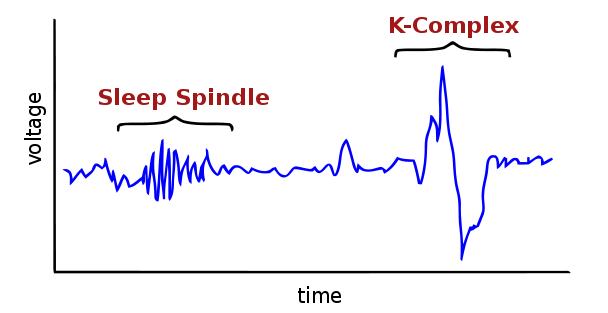
\includegraphics[width=\textwidth, trim={6em 6em 0 0}, clip]{sleep_spinddle}
        \column{.35\columnwidth}
        \visible<2->{
            \highlightbox{
                \centering \Large
                Neural signals exhibit
                diverse and complex
                morphologies
            }
        }
    \end{columns}
    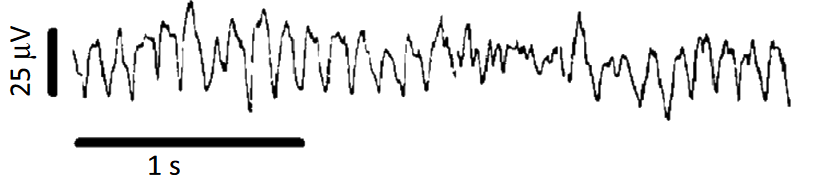
\includegraphics[width=\textwidth]{mu_rythm}\\[-1.5em]
    \rightcite{S. Cole, B. Voytek (2017) Trends in Cognitive Sciences}
    \vskip-7em
        \begin{columns}[c]
        \column{.7\columnwidth}
        \visible<3->{\highlightbox{\vskip.1em
        \Large Waveform shape is related to disease\\
        \eg{} Parkinson \rightcite{Jackson et al. (2019)}}\\[.3em]}
        \end{columns}
    \vskip3em
    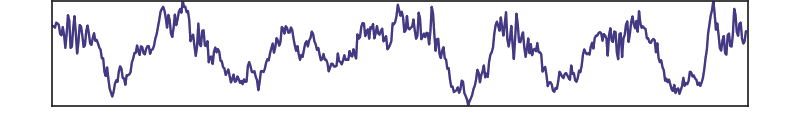
\includegraphics[width=\textwidth]{cfc}\\[-.8em]
    \rightcite{\footnotesize Dupré la Tour, Tallot, Grabot, Doyère, van Wassenhove, Grenier, Gramfort\\
    \hfill (2017) PLOS Computational biology}
}

\frame{
        \frametitle{"Textbook" brain rythm \rightcite{According to Alex!}}

        \centering
        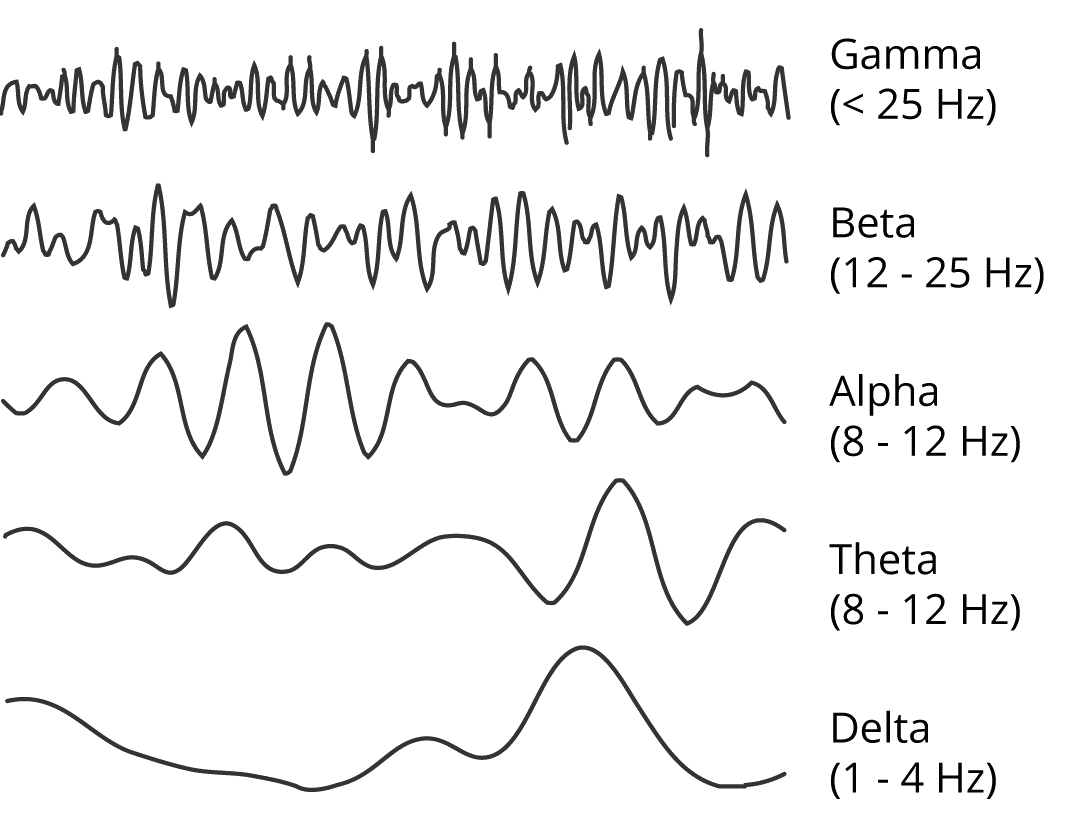
\includegraphics[width=.8\textwidth]{brain_rythm}

}


\frame{
    \frametitle{Linear filtering}

    After Linear filters, everything looks like a sinusoïd.
    {\centering
    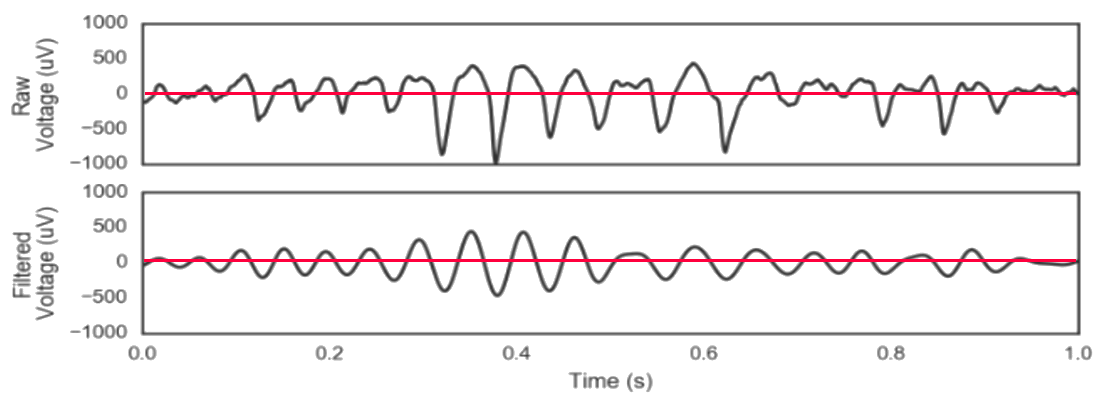
\includegraphics[width=.9\columnwidth]{filtering_mu_waves}\\[1em]
    $\Rightarrow$ Lose the asymmetry and the shape information.
    }

}

\frame{
    \frametitle{Fourier Fallacy}
    \large
    {\centering
    "Even though it may be possible to analyze the complex forms of brain waves into a {\bf number of different sine-wave} frequencies, this may lead only to what might be termed a “{\bf Fourier fallacy}”, if one assumes {\bf ad hoc} that all of the necessary frequencies actually occur as periodic phenomena in {\bf cell groups} within the brain."\\[.5em]}
    \rightcite{Jasper (1948)}
    \vskip.5em
    \visible<2->{
        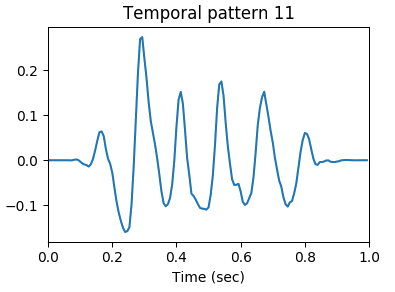
\includegraphics[width=.5\textwidth]{mu_waveform}%
        \alt<3>{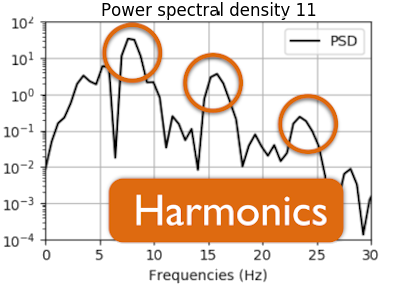
\includegraphics[width=.5\textwidth]{mu_waveform_harmonic}}
               {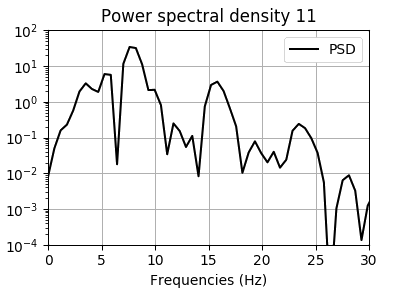
\includegraphics[width=.5\textwidth]{mu_waveform_psd}}
    }

}

\section{Can't we learn the waveforms?}
\parttitleframe{}

\frame[t]{
    \frametitle{Local structure in signals}
    \vskip1.5em%
    \centering%
    \only<1>{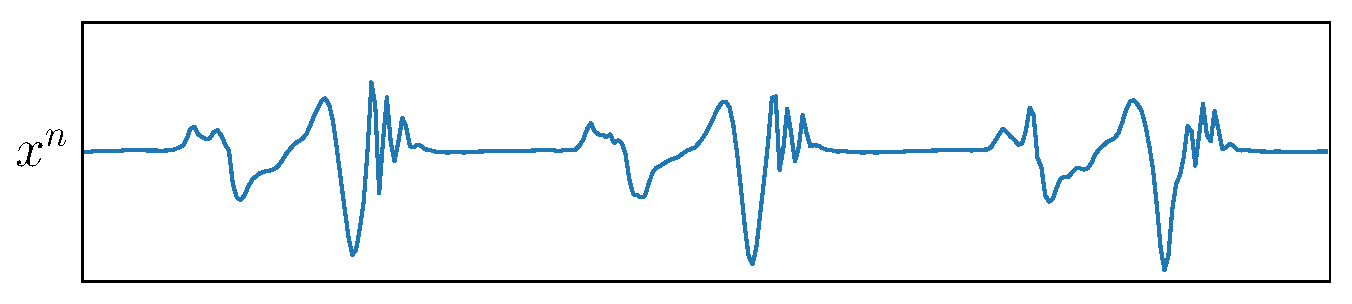
\includegraphics[width=\textwidth]{intro_csc_0}}%
    \only<2>{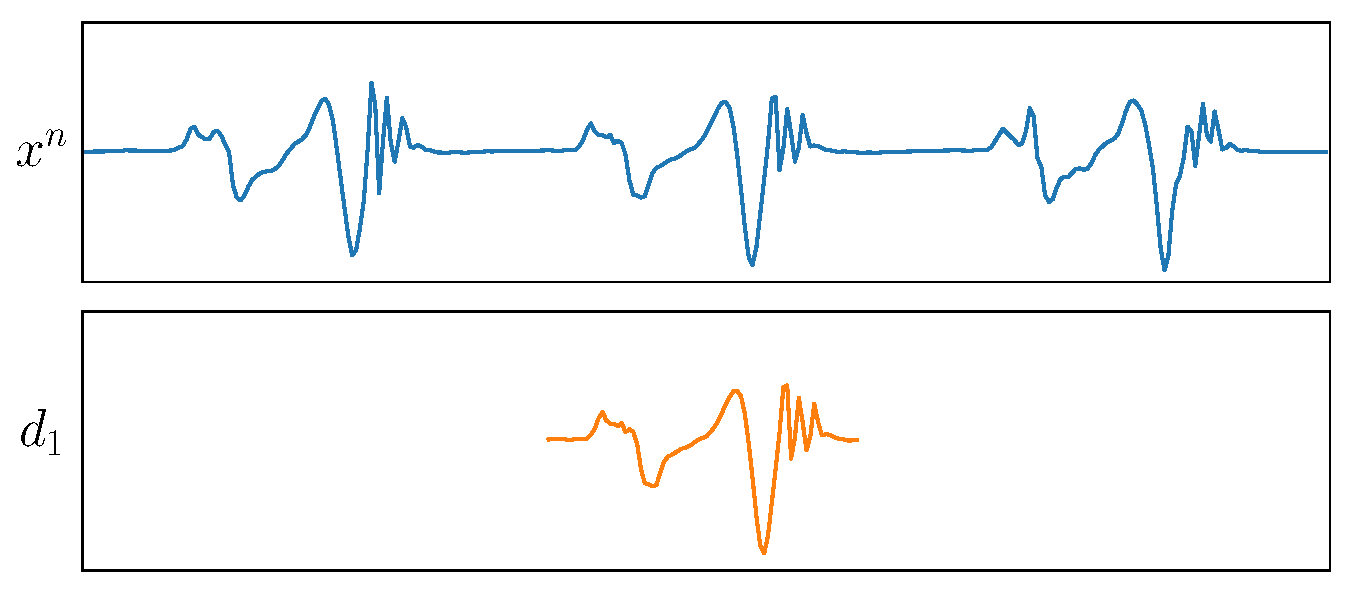
\includegraphics[width=\textwidth]{intro_csc_1}}%
    \only<3>{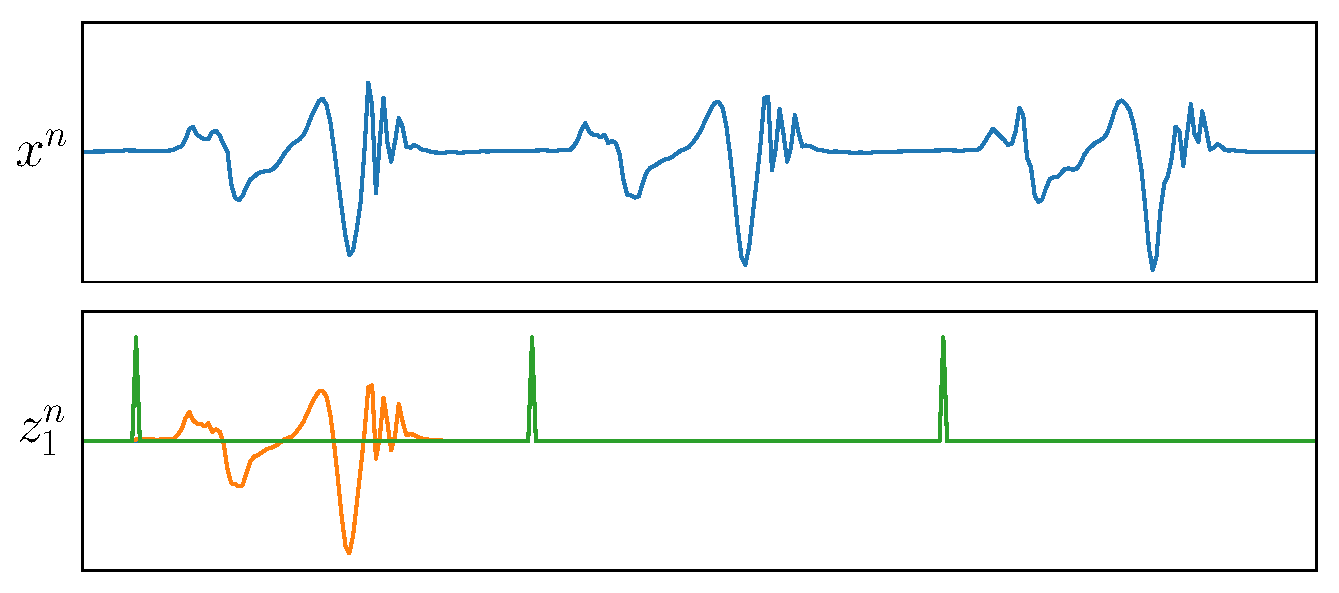
\includegraphics[width=\textwidth]{intro_csc_2}}%
    \only<4>{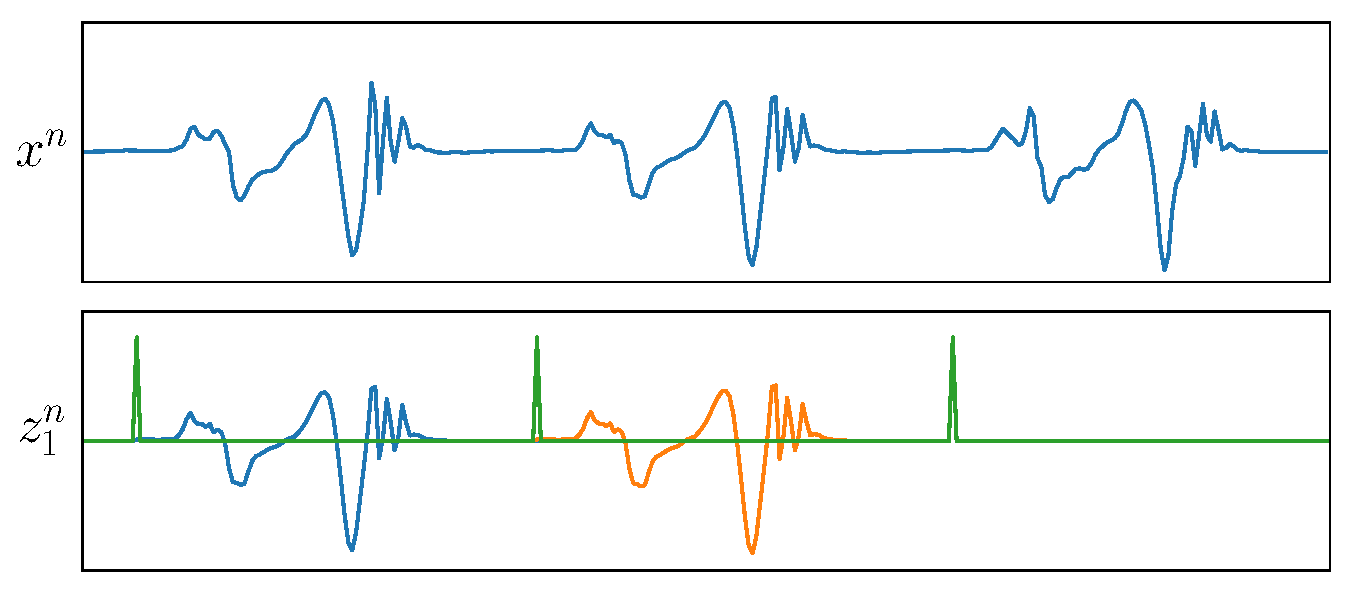
\includegraphics[width=\textwidth]{intro_csc_3}}%
    \only<5>{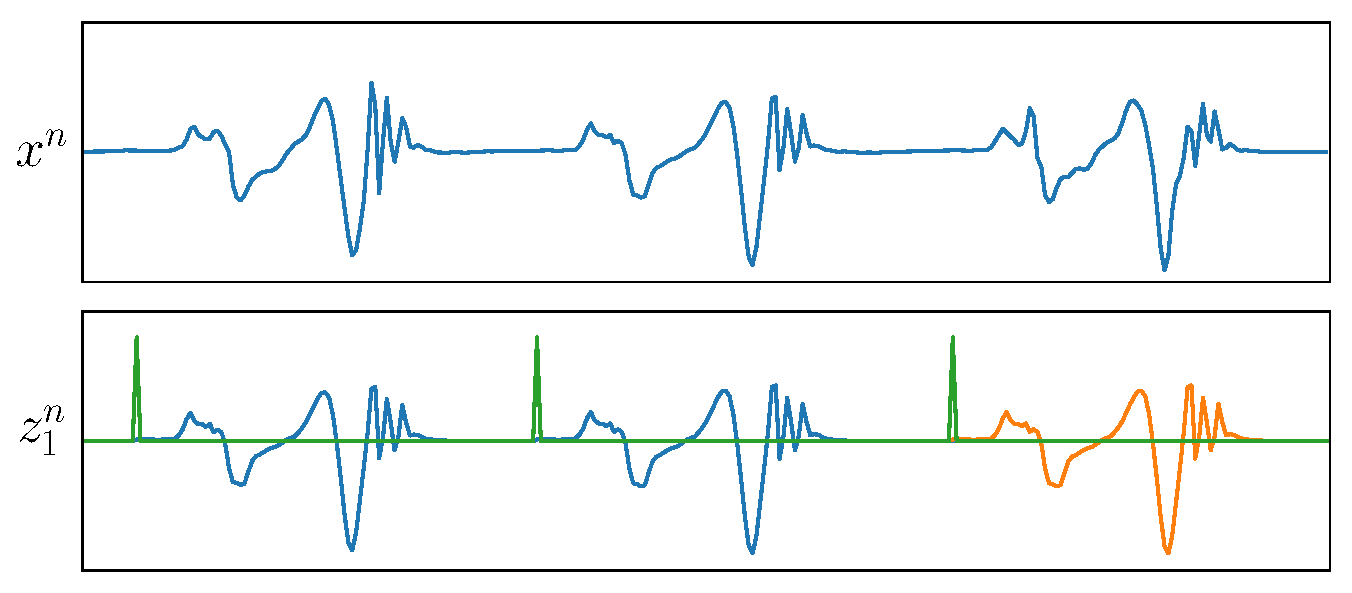
\includegraphics[width=\textwidth]{intro_csc_4}}%
    \only<6->{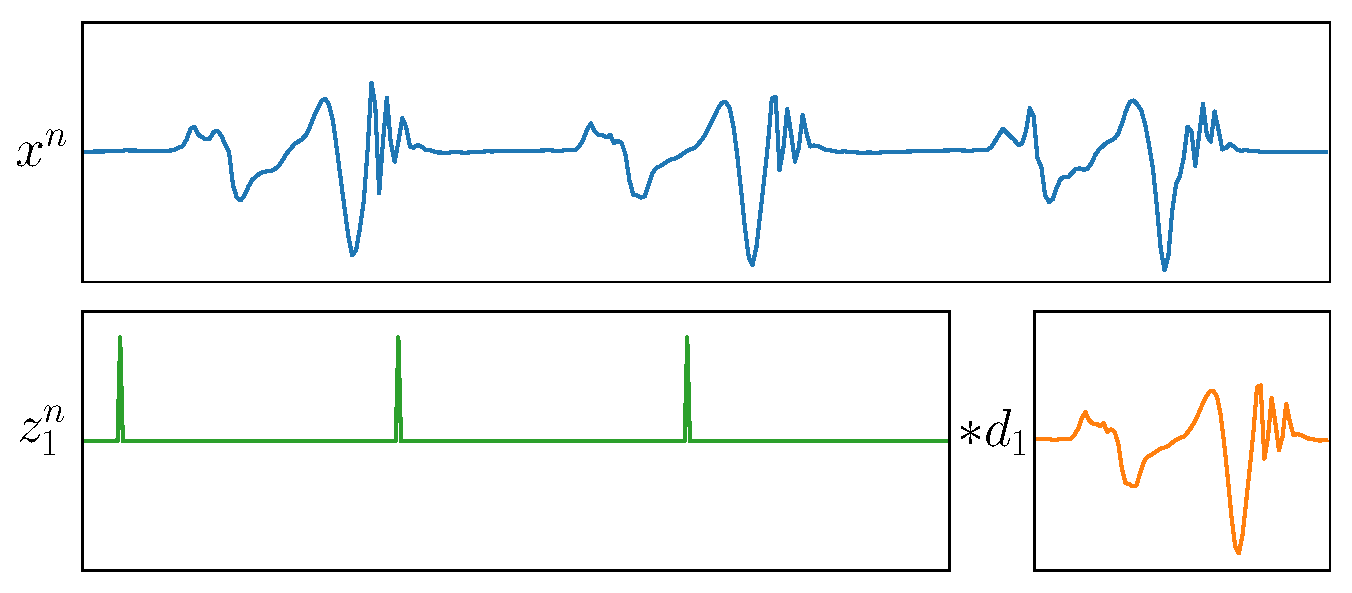
\includegraphics[width=\textwidth]{intro_csc_5}}%
    \vskip.2em%
    \only<7>{%
        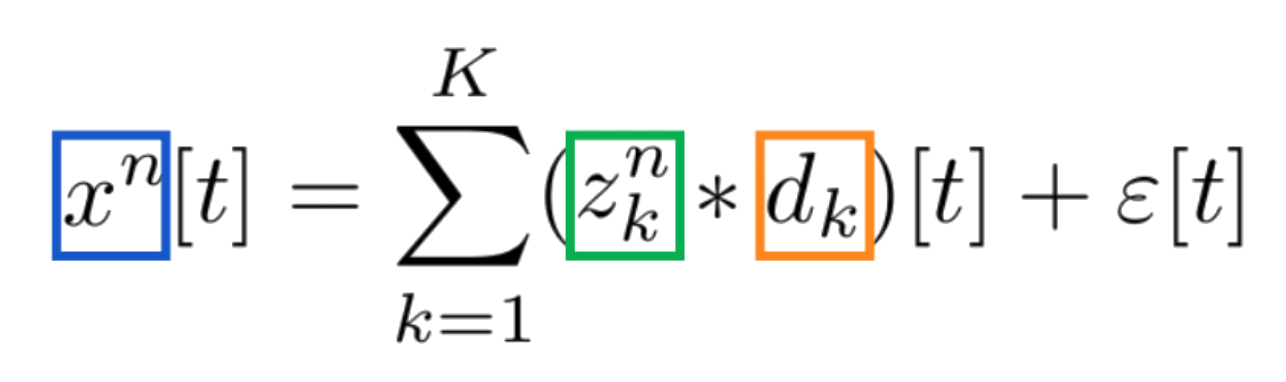
\includegraphics[width=.6\textwidth]{csc_explain_eq_color}%
    }
}

\frame{
    \frametitle{Learned atoms \rightcite{Jas et al. (2017)}}
    \begin{columns}[T]
        \column{.2\columnwidth}
            \flushright \Large Data:
        \column{.8\columnwidth}
            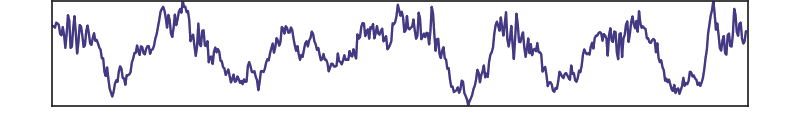
\includegraphics[width=\columnwidth]{cfc}
    \end{columns}
    \begin{columns}[c]
        \column{.5\columnwidth}
            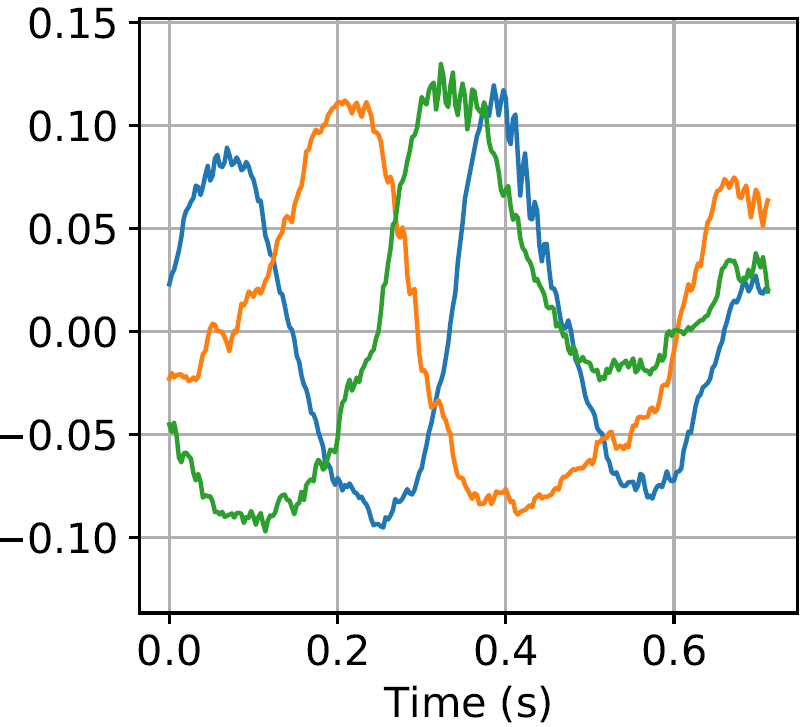
\includegraphics[width=\columnwidth]{learned_cfc}
        \column{.1\columnwidth}
        \column{.3\columnwidth}
            \visible<2>{
            \highlightbox{
                \centering
                \Large What to do\\in the case of\\multivariate signals?
            }}
        \column{.1\columnwidth}


    \end{columns}
}

\frame[t]{
    \frametitle{EM wave diffusion}
    \begin{itemize}
    \uncover<1->{\item Recording here with 8 sensors}
    \uncover<2->{\item EM activity in the brain}
    \uncover<3->{\item The electric field is spread \textbf{linearly} and \textbf{instantaneously} over all sensors (Maxwell equations)}
    \end{itemize}
    \centering
    \only<1>{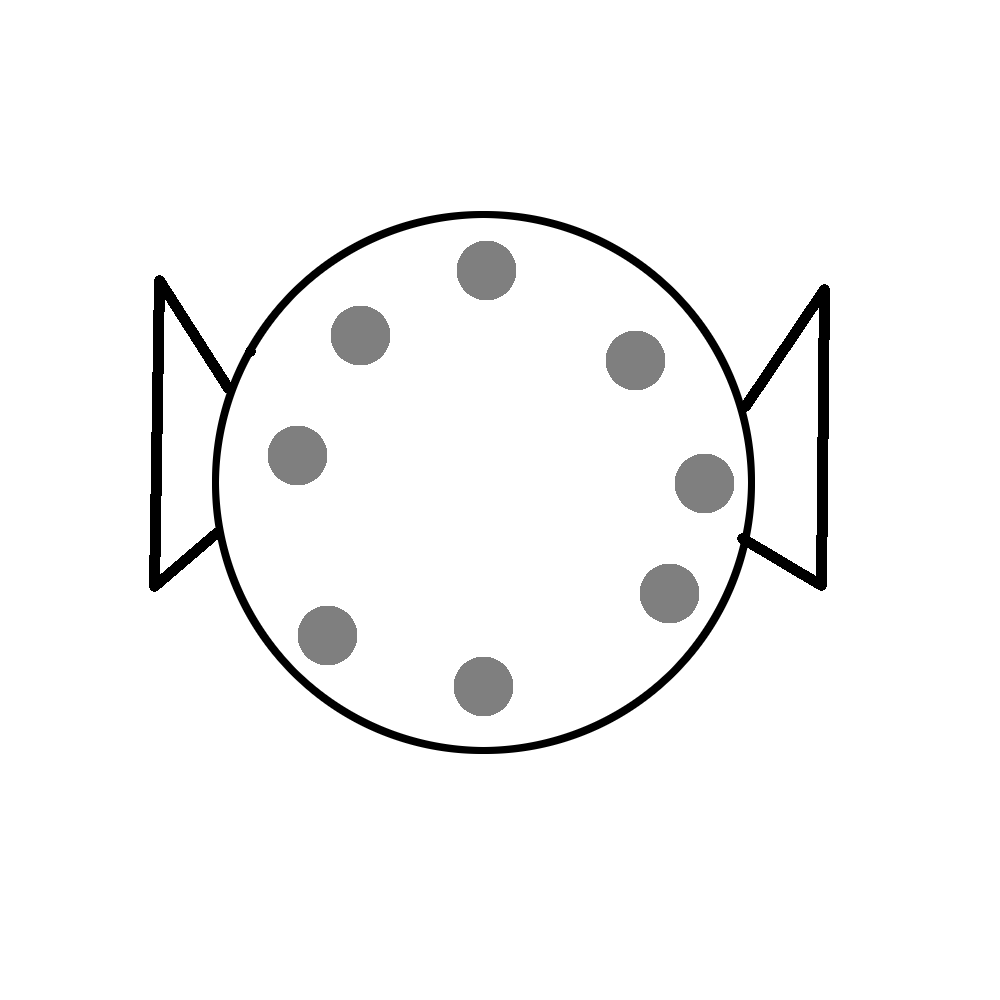
\includegraphics[width=.5\textwidth]{physic1}}%
    \only<2>{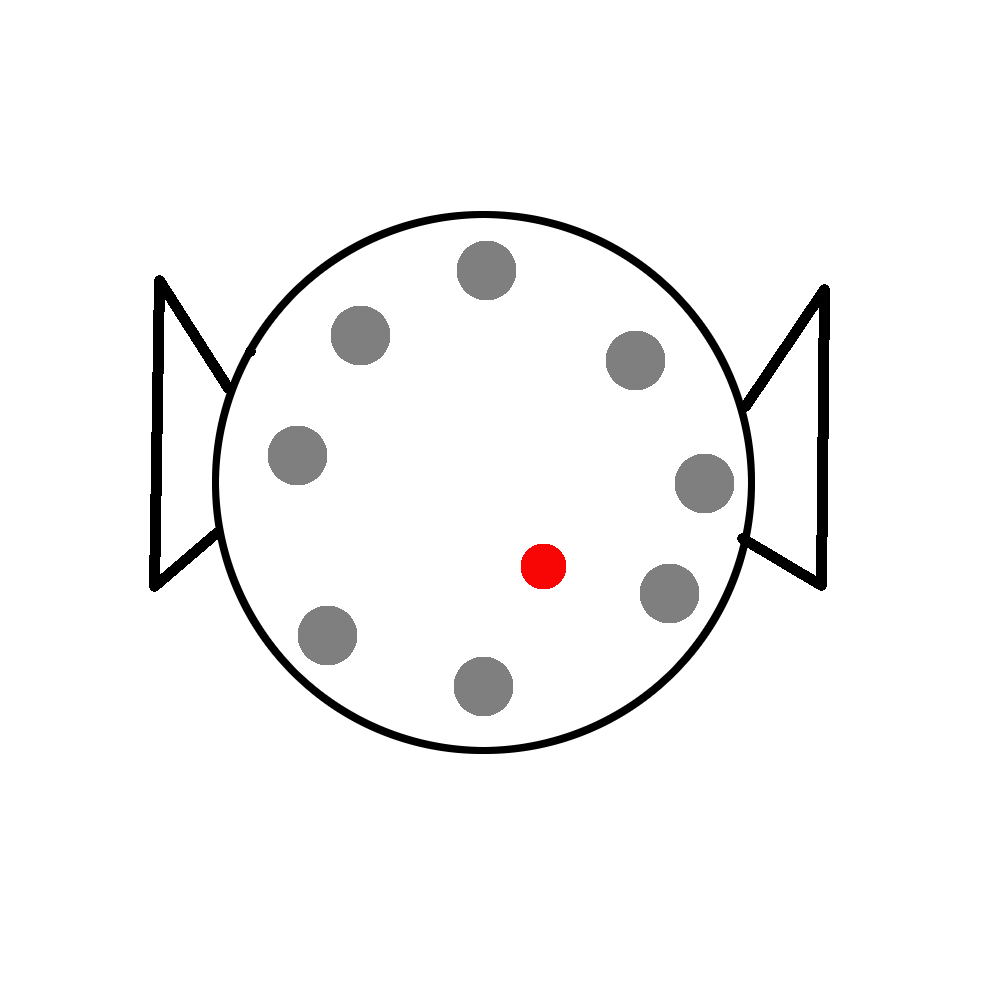
\includegraphics[width=.5\textwidth]{physic2}}%
    \only<3>{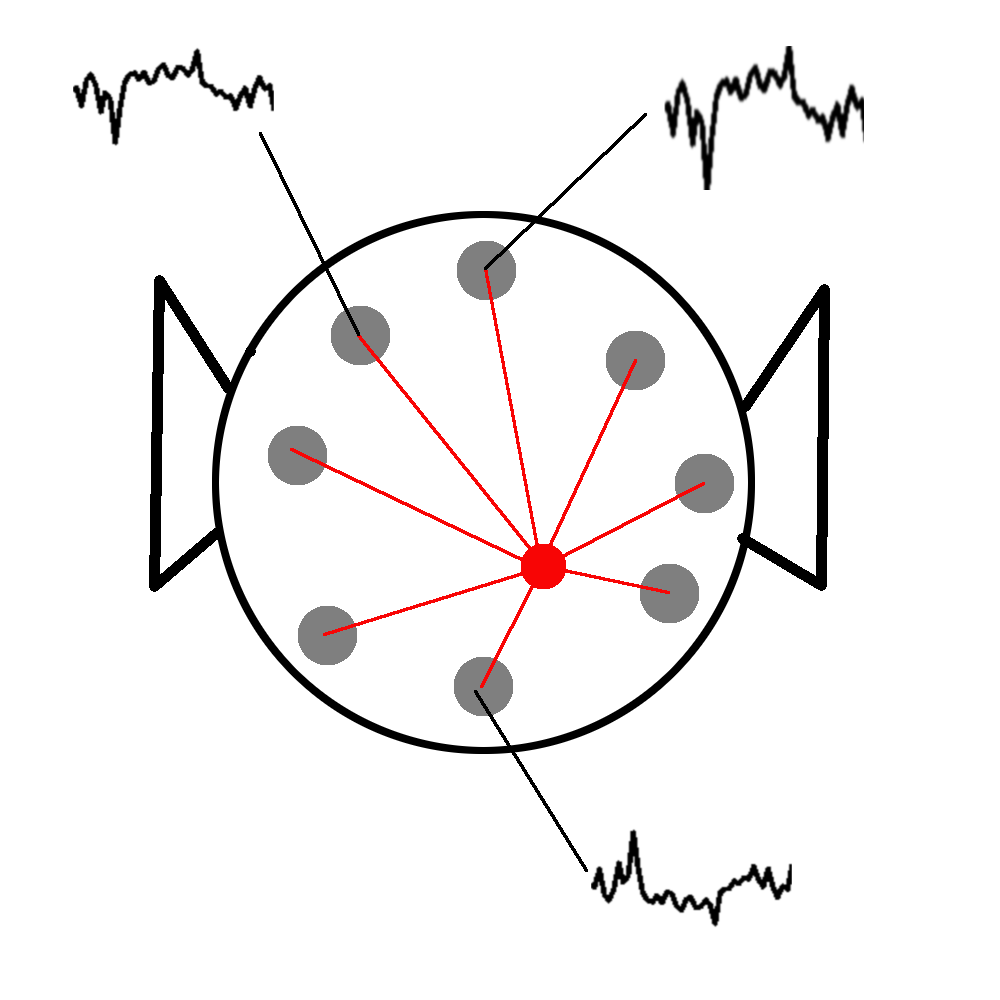
\includegraphics[width=.5\textwidth]{physic3}}%
    \only<4>{\vskip1em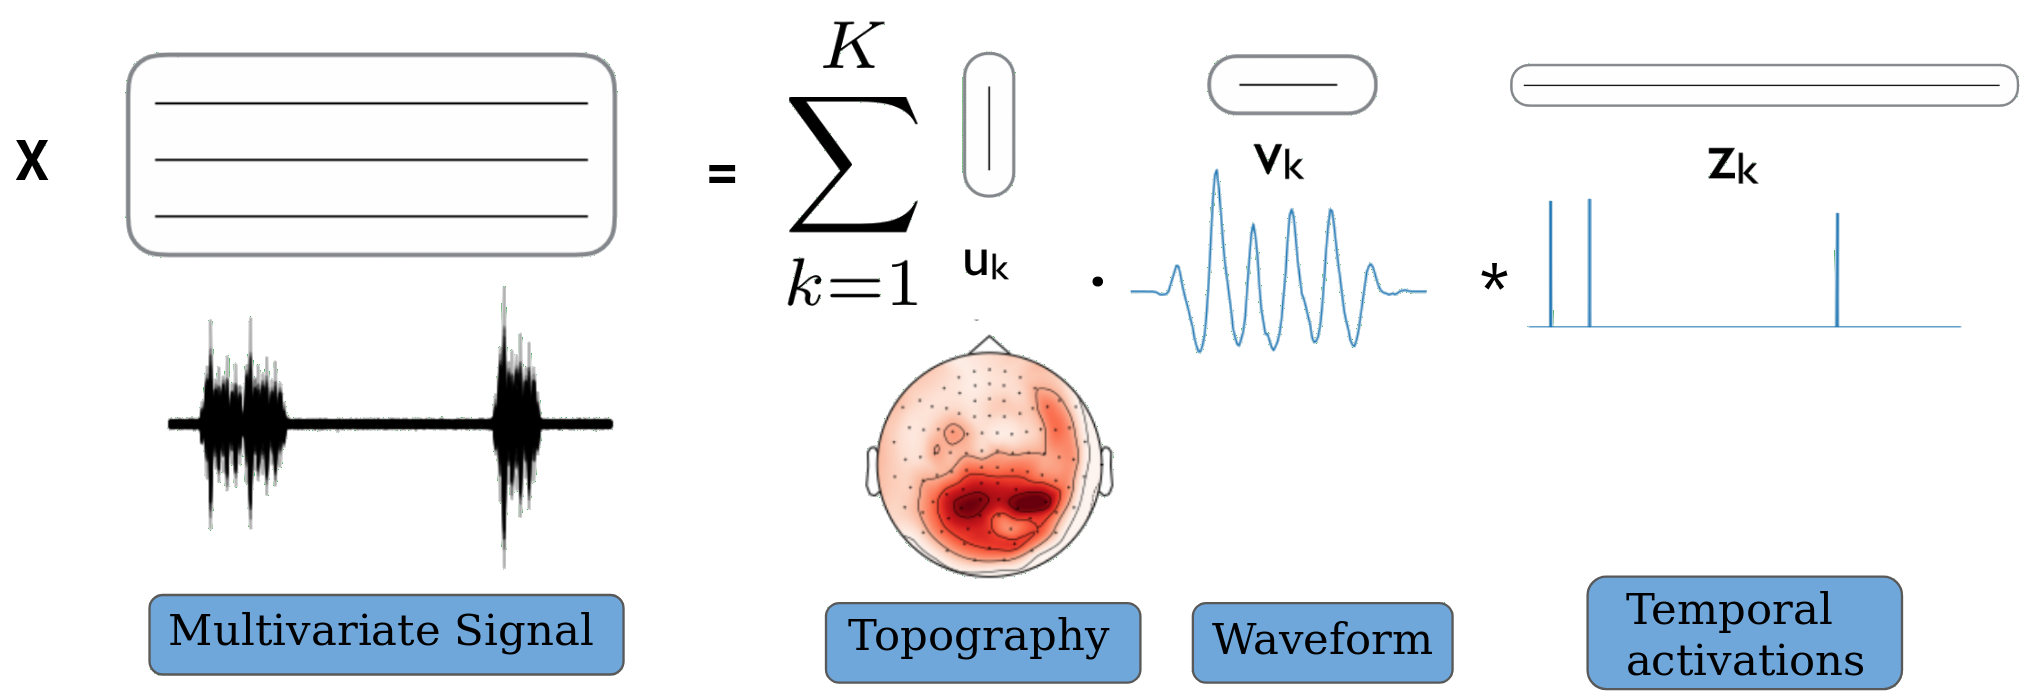
\includegraphics[height=.45\textheight]{rank1}}
}

\frame[t]{
    \frametitle{Learned atoms -- Artifacts}

    \centering
    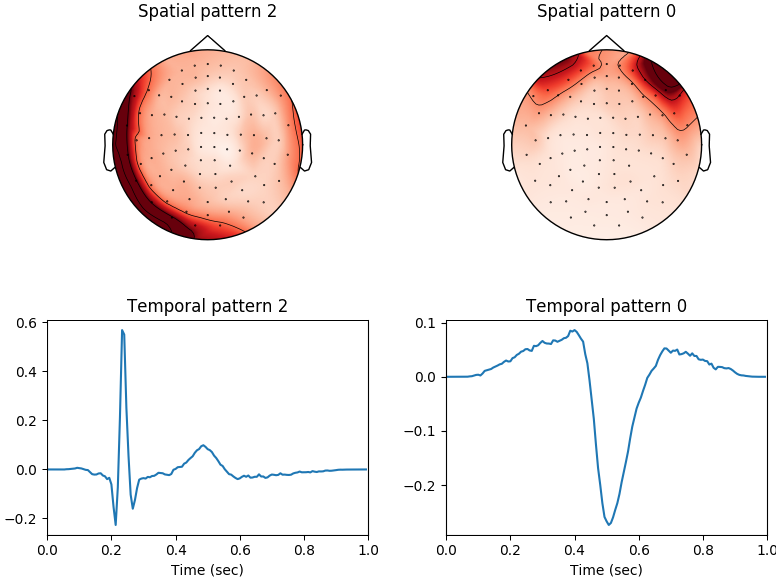
\includegraphics[width=.9\columnwidth]{artifacts}
}
\frame[t]{
    \frametitle{Learned atoms -- Evoked response}

    \centering
    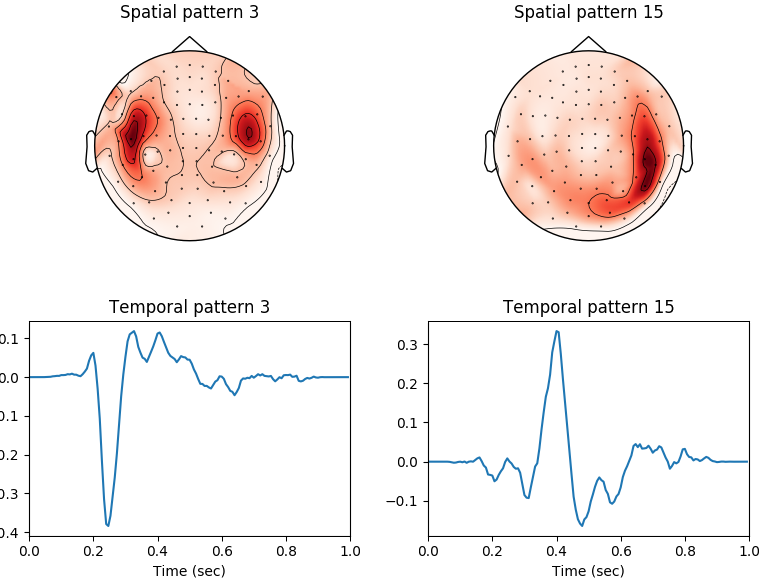
\includegraphics[width=.9\columnwidth]{evoked}
}
\frame[t]{
    \frametitle{Learned atoms -- Evoked response}

    \centering
    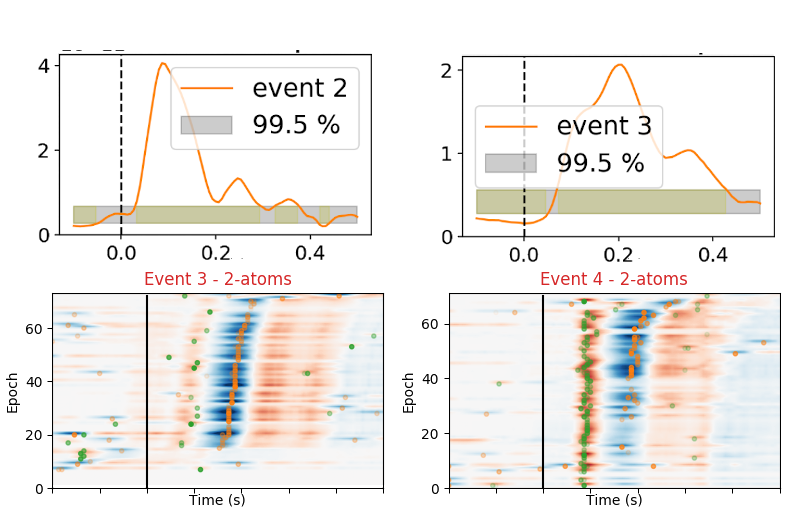
\includegraphics[width=.9\columnwidth]{activations}
    \vskip-12em
    \visible<2>{
    \begin{columns}
        \column{.4\columnwidth}
        \highlightbox{\centering \Huge Work in progress!}
    \end{columns}
    }

}
\frame[t]{
    \frametitle{Learned atoms -- Complex waveforms}

    \centering
    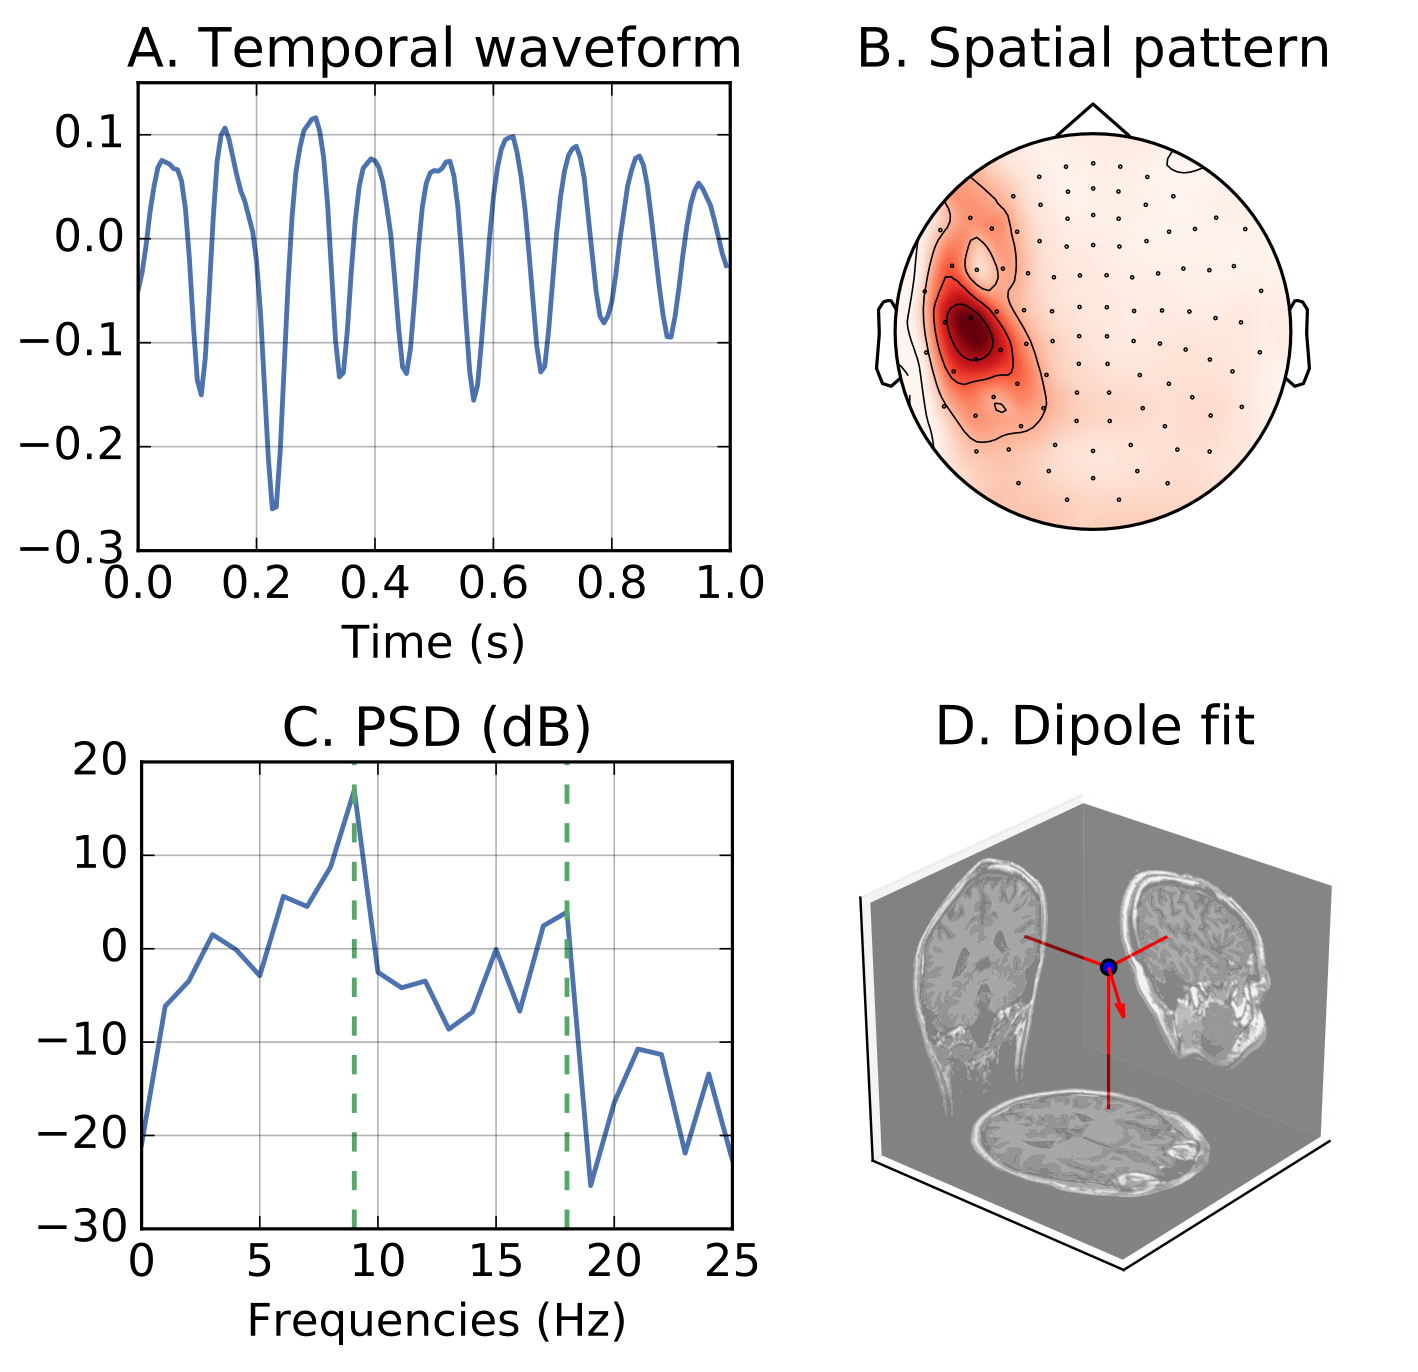
\includegraphics[width=.7\columnwidth]{atom_somato}
}

{\usebackgroundtemplate{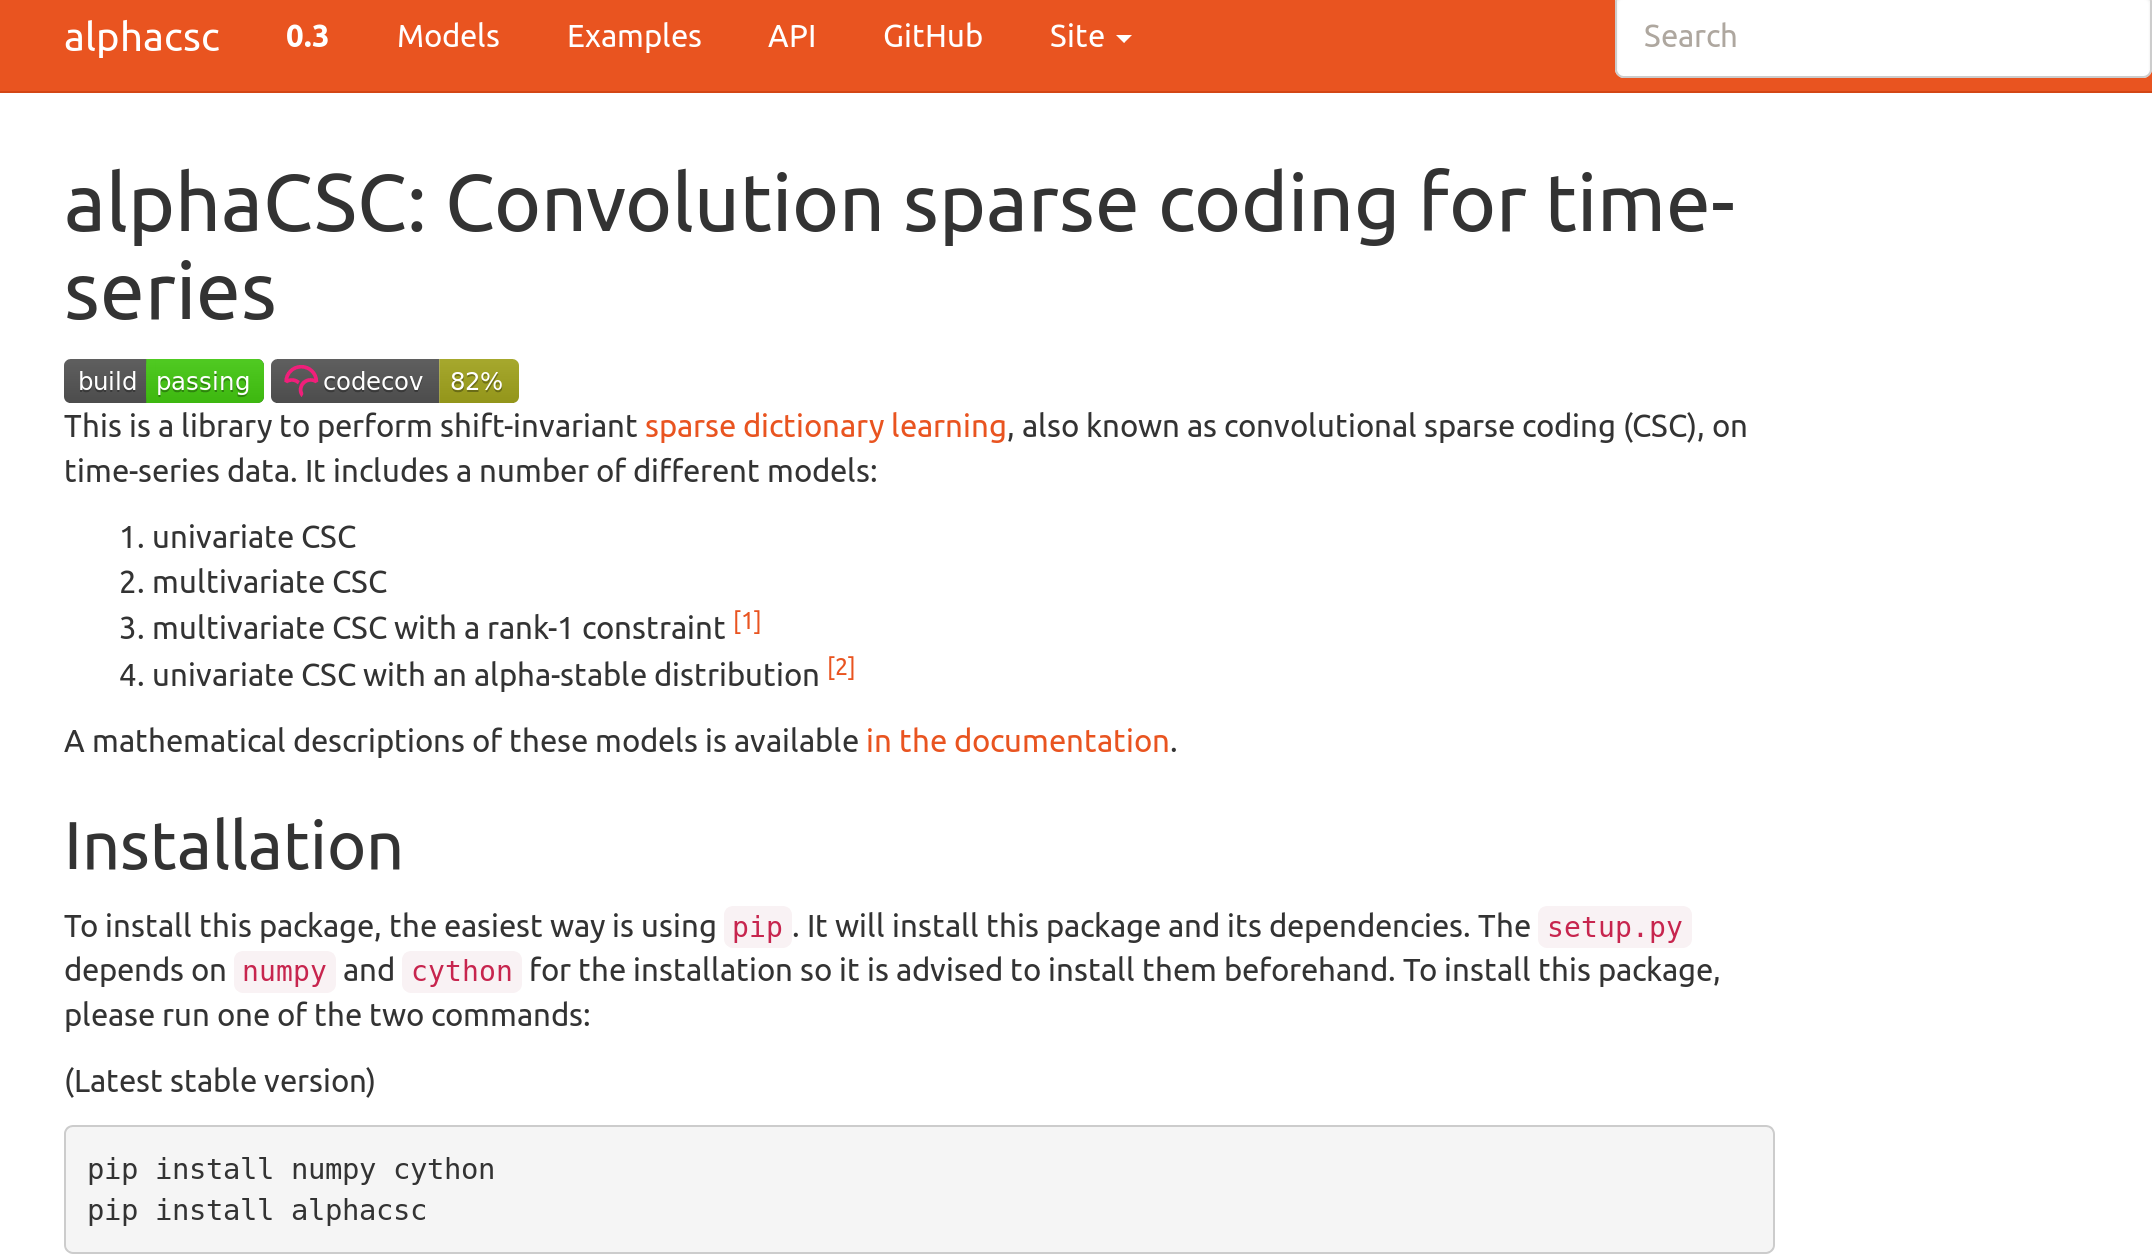
\includegraphics[width=\paperwidth]{alphacsc}}%
\frame{
    \visible<2->{
        \begin{columns}
            \column{.5\textwidth}
            \column{.4\textwidth}
            \highlightbox{Python code online:\\
                          https://alphacsc.github.io\\[1em]
                          \texttt{pip install alphacsc}}
            \vskip2em
            \visible<3>{
                \highlightbox{Examples reproduce figures from this talk!}
            }

        \end{columns}
    }
}}

%===========================================================================
\section{R}
%===========================================================================

\begin{frame}{Recurring Patterns extraction}
    \textbf{Convolutional Dictionary Learning}
    \begin{itemize}\itemsep.5em
        \item Flexible pattern extraction technique,
        \item Computationally tractable for more and more problems,
        \item Some application are already beginning to emerge.
    \end{itemize}
    \vskip2em
    \textbf{Challenges}
    \begin{itemize}\itemsep.5em
        \item Theoretical challenges remains (convergence, recoverability),
        \item The evaluation (and thus the parameter choices) is still not clear,
        \item Can give some insight for deep learning models?
    \end{itemize}
\end{frame}


\frame[t]{
\frametitle{Going further: capturing temporal}
\begin{columns}[T]
    \column{.5\textwidth}
        \centering
        \textbf{How to highlight temporal dependency?}

        \vskip1em
        \centering
        \setlength\bodywd{.9\linewidth}
        \highlight[wd=\bodywd]{Model inter-atom interactions:}

        \raggedright\vskip1.5em
            Pénalité $\ell_1$\\[.3em]
            \hskip2ex$\Rightarrow$ independent activations\\[1em]
        \uncover<2->{Group penalty (\eg{} $\ell_{1, 2}$)\\[.3em]
            \hskip2ex$\Rightarrow$ simultaneous activations\\[1em]}
        \uncover<3->{Point process ponctuels (\eg{} Hawkes)\\[.3em]
            \hskip2ex$\Rightarrow$ temporal interactions\\[1em]}

    \column{.5\textwidth}
        \centering%
        \setlength\bodywd{.8\linewidth}
        \only<1>{

            \highlight[c=linkcolor, wd=\bodywd]{Independent activations}\\[1em]
            \includegraphics[height=8em]{connectivity_independent.png}
            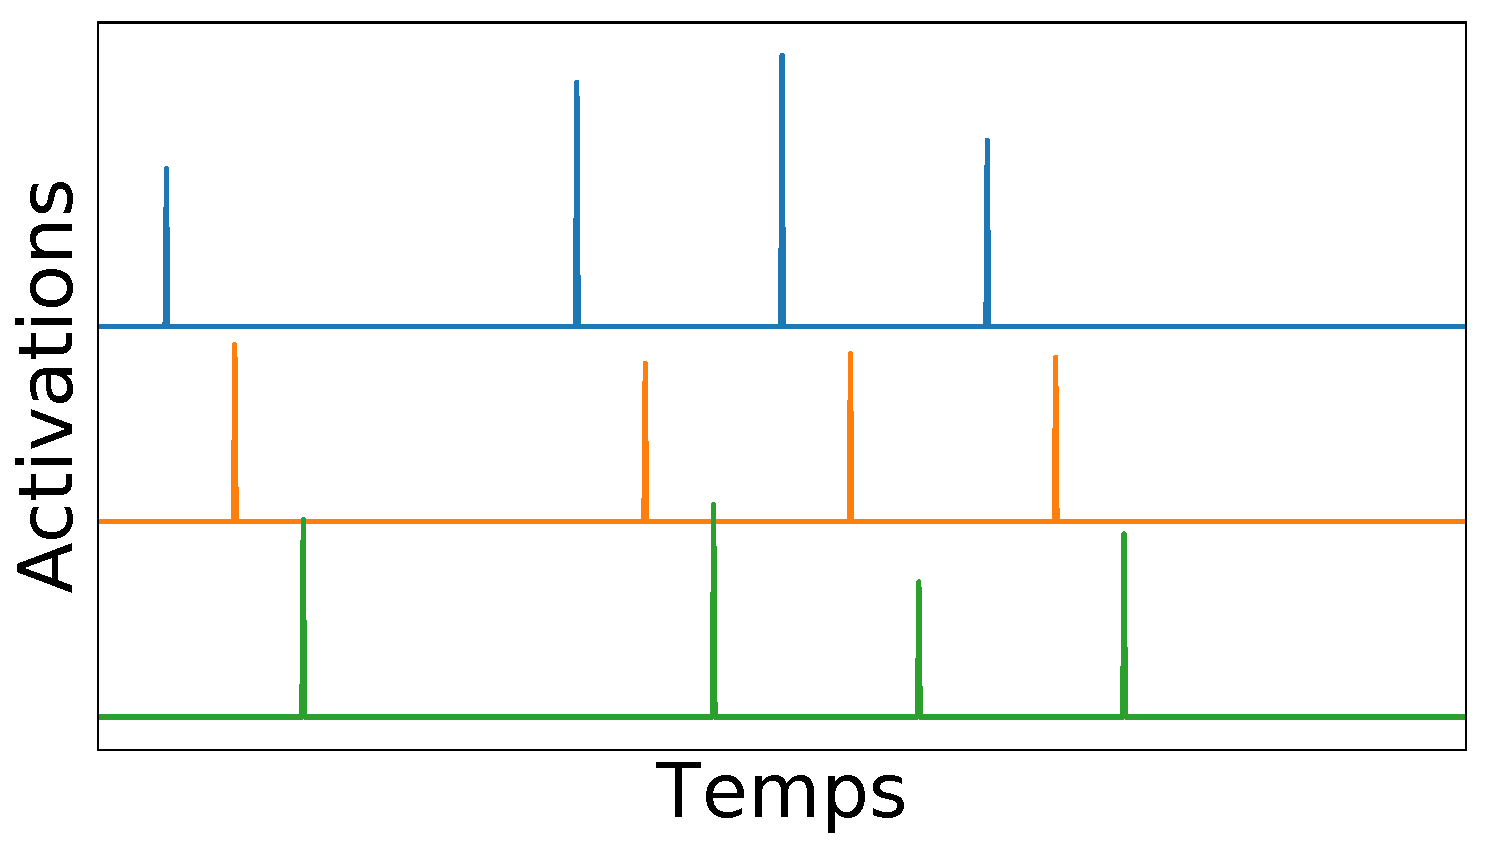
\includegraphics[width=\linewidth]{time_dependency}
        }%
        \only<2>{
            \highlight[c=linkcolor, wd=\bodywd]{Simultaneous activations}\\[1em]
            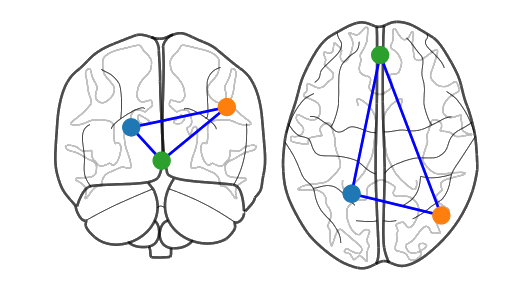
\includegraphics[height=8em]{connectivity_simultaneous.png}
            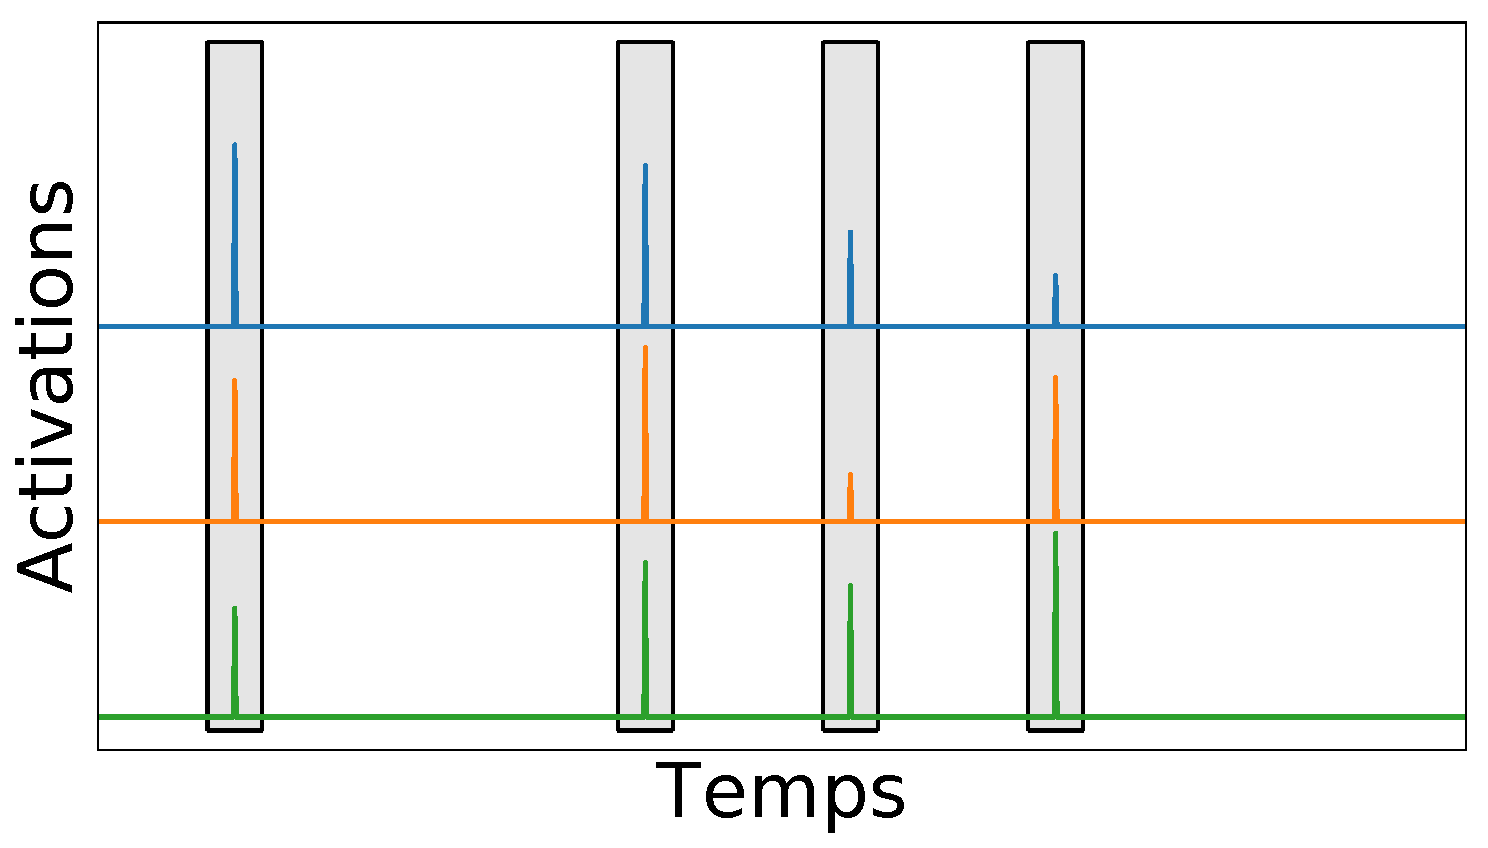
\includegraphics[width=\linewidth]{time_dependency_simultaneous}
        }%
        \only<3>{
            \highlight[c=linkcolor, wd=\bodywd]{Temporal interactions}\\[1em]
            \includegraphics[height=8em]{connectivity_default_mode.png}
            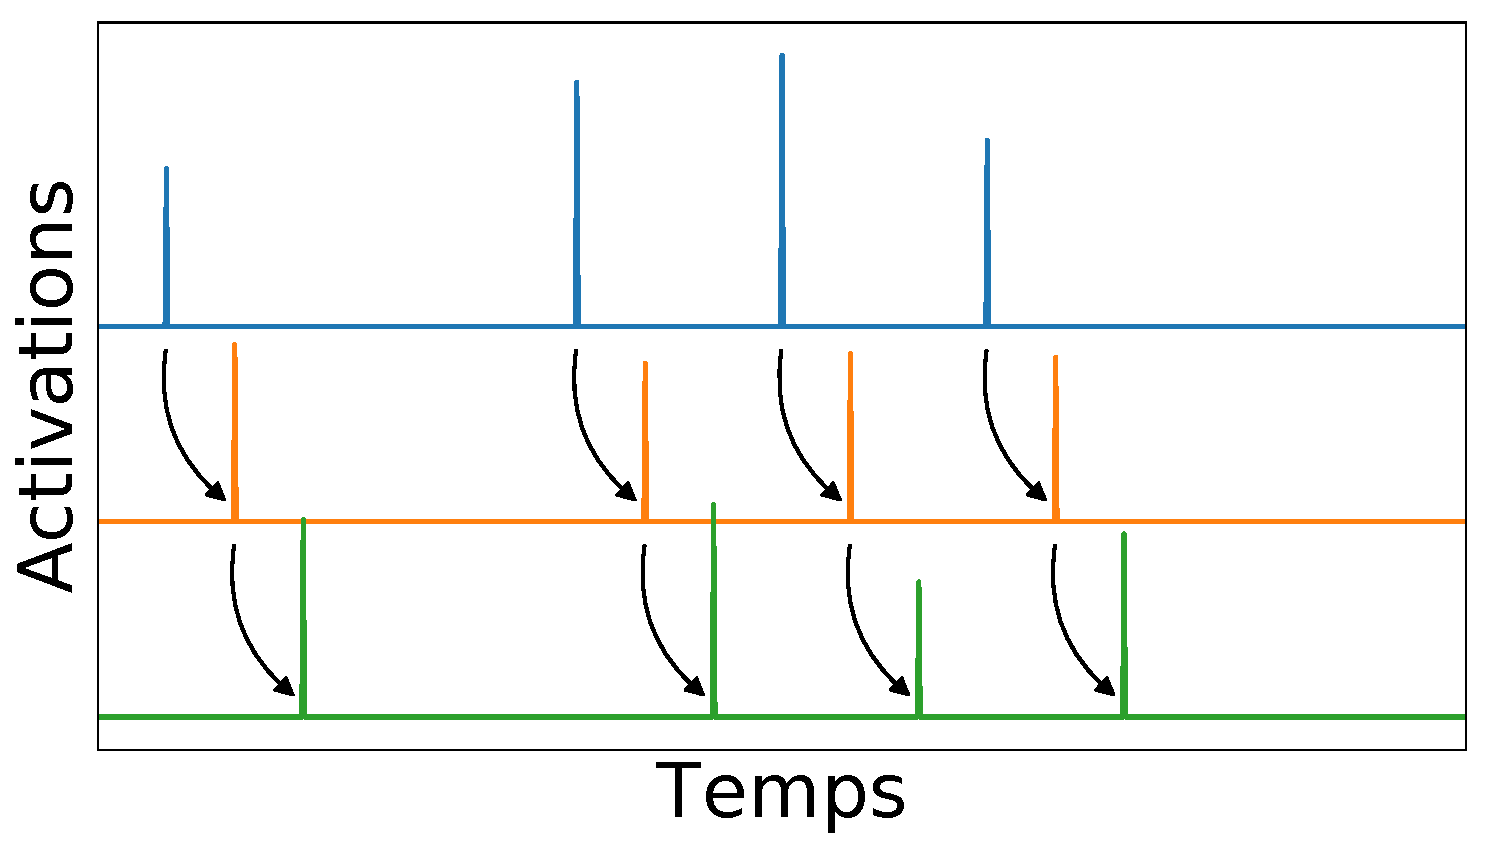
\includegraphics[width=\linewidth]{time_dependency_arrow}
        }%
    \end{columns}

}


\frame[t]{
    \frametitle{Deep Learning for Inverse problem}

    \centering
    \definecolor{Z}{RGB}{45,162,65}
    \definecolor{F}{RGB}{180,35,35}
    \begin{tikzpicture}
        \node (meg) {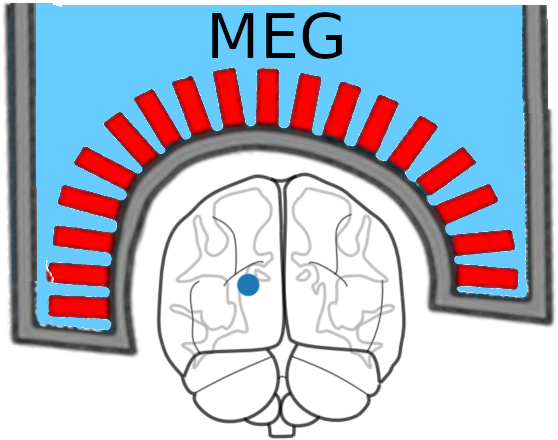
\includegraphics[width=9em]{meg_localised_source}};
        \draw[->, thick] ($(meg.east) - (0, 1.5em)$) -- ++(5em, 0)
            node[midway, align=center] (maxwell) {\small Maxwell\\ \small equations}
            node[right] (topomap) {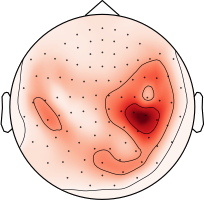
\includegraphics[width=4em]{topomap_somato}};
        \draw[->, thick] (topomap.east) -- ++(5em, 0)
            node[midway, align=center] {\small Inverse\\ \small Problem}
            node[right] (brain) {\includegraphics[width=4em]{brain_activity}};
            \node[draw, rounded corners, above=2.5em] at (topomap.center) {
                \color{linkcolor} $\pmb X$};
            \node[draw, rounded corners, above=2.5em] at (brain.center) {
                \color{Z} $\pmb Z$};
            \node[draw, rounded corners, above=2.5em] at (maxwell.center) {
                \color{F} $\pmb F$};
    \end{tikzpicture}

    {\bf Inverse Problem:} $\argmin_{\color{Z} \pmb Z} \|{\color{linkcolor} \pmb X}
                        - {\color{F} \pmb F}{\color{Z} \pmb Z}\|_2^2
                        + \mathcal R({\color{Z} \pmb Z})$\\[2em]

    \begin{itemize}\itemsep1em
        \item Fast iterative solvers to compute {\color{Z} $\pmb Z$}
        \rightcite{Massias et al. (2017)}
        \item Use of deep learning to inverse this system\\
        \rightcite{Moreau et al. (2017); Ablin et al. (2019)}
    \end{itemize}

}


\begin{frame}{}
\vskip2em
{\centering
    \usebeamercolor[fg]{title}
    \usebeamerfont{title}
    \Huge \bf Thanks!\\[2em]}

Code available online:\\[1em]


\includegraphics[height=.8em]{github}~\textbf{alphacsc} :  \url{alphacsc.github.io}\\[2em]

Slides are on my web page:\\[1em]
\hskip5em\includegraphics[height=.8em]{website} \url{tommoral.github.io}
\hskip4em 
\includegraphics[height=.8em]{twitter} \href{https://twitter.com/tomamoral}{@tomamoral}


\end{frame}

\end{document}
